\documentclass[a4paper,12pt]{article}
\usepackage{times}
\usepackage[francais]{babel}
\usepackage[utf8]{inputenc}
\usepackage[T1]{fontenc}
\usepackage{amsmath}
\usepackage{amssymb}
\usepackage{graphicx}
\usepackage{pdfpages}
\usepackage{pdflscape}
\usepackage{listings}
\usepackage{longtable}
\usepackage{hyperref}
\lstset{literate=
{é}{{\'e}}1
{è}{{\`e}}1
{ê}{{\^e}}1
{à}{{\`a}}1
{â}{{\^a}}1
}
\lstset{language=C++,
                basicstyle=\footnotesize,
                keywordstyle=\footnotesize\color{blue},
                otherkeywords={override,nullptr}
}
\definecolor{orange}{rgb}{0.8,0.4,0.0}
\definecolor{darkblue}{rgb}{0.0,0.0,0.6}
\definecolor{cyan}{rgb}{0.0,0.6,0.6}
\lstdefinelanguage{JSON}
{
  basicstyle=\normalsize,
  columns=fullflexible,
  showstringspaces=false,
  commentstyle=\color{gray}\upshape,
  morestring=[b]",
  morestring=[s]{>}{<},
  morecomment=[s]{<?}{?>},
  stringstyle=\color{orange},
  identifierstyle=\color{darkblue},
  keywordstyle=\color{blue},
  morekeywords={string,number,array,object}% list your attributes here
}

\sloppy

\setlength{\topmargin}{0cm}
\setlength{\headsep}{0.in}
\setlength{\headheight}{0.in}
\setlength{\evensidemargin}{0cm}
\setlength{\oddsidemargin}{-1cm}
\textwidth 18cm
\textheight 25cm

\begin{document}

\thispagestyle{empty}

\begin{titlepage}

\vspace*{2cm}

\begin{center}\textbf{\Huge Projet Logiciel Transversal}\end{center}{\Large \par}

\begin{center}\textbf{\large Alexandre Génot - Anthony Peloille}\end{center}{\large \par}

\vspace{2cm}

\begin{figure}[h]
\begin{center}
\includegraphics[width=\textwidth]{slaythespire.jpg}
\caption{\label{Slay the Spire}Slay the Spire}
\end{center}
\end{figure}

\clearpage

{\small
\tableofcontents
}

\end{titlepage}

\clearpage
\section{Présentation Générale}

\subsection{Archétype}

Les mécaniques du jeu s'inspirent de The Legend of Zelda (1986) qui est un jeu de type action/aventure.

\subsection{Règles du jeu}

Le joueur évolue dans un donjon dont la structure des étages est générée aléatoirement. A chaque étage il doit atteindre un boss, pour cela il se déplace de case en case à la manière d’un jeu de plateau. Les cases peuvent contenir différents types d'évènements : combat, récompense, bonus, malus.... Le but est de sortir du donjon en ayant complété chaque étage, c'est-à-dire avoir vaincu chacun des boss. 
Les phases de combats se déroulent se forme de combats tour par tour, à chaque tour le personnage peut attaquer (différents coups d'épée) puis le tour suivant, l'ennemi attaque. Chaque personnage (personnage principal ou ennemi) dispose de 3 caractéristiques :
- Les points de vie/Health Points, lorsque ceux-ci arrivent à 0 le personnage meurt. 
- L'attaque , conditionne les dégâts qu'inflige un coup.
- La défense, détermine la quantité de point de vie perdue après avoir reçu une attaque.
Le système de combat est basé sur l’utilisation de cartes permettant au joueur d’affronter ses adversaires (le nombre d’adversaires augmente au cours du jeu). Les cartes sont obtenues en récompenses de combat, au magasin ou lors d’évènements aléatoires. Le personnage peut trouver de l’équipement lui permettant d’augmenter ses statistiques (vie, armure, puissance).

\subsection{Ressources}

\begin{figure}[h]
\begin{center}
\includegraphics[width=0.5\textwidth]{dungeontile.png}
\caption{\label{tiles}Tuiles du décor et personnages}
\end{center}
\end{figure}

\begin{figure}[h]
\begin{center}
\includegraphics[width=0.5\textwidth]{card.png}
\caption{\label{card}Template de carte utilisé lors des combats}
\end{center}
\end{figure}

\begin{figure}[h]
\begin{center}
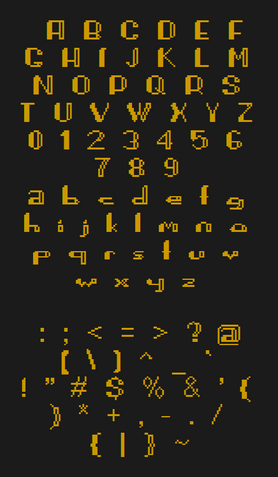
\includegraphics[width=0.5\textwidth]{font.png}
\caption{\label{font}Police de caractères}
\end{center}
\end{figure}

\clearpage
\section{Description et conception des états}

\subsection{Description des états}

Pour chacun des états du jeu, on retrouve une combinaison d'éléments fixes (la structure du labyrinthe) et d'éléments mobiles (personnage principal et ennemis).
Pour chaque élément, on comptera 2 propriétés que sont sa position et son identifiant (un id pour les murs, un pour les ennemis, le personnage principal ...).

\subsubsection{État éléments fixes}

Chaque étage du donjon possède un certain nombre fixe de cases. Toutes les cases ont un type parmi ces 4 : Mur, Espace (vide), Porte, Coffre.

Cases "Mur" (Wall) : Elles servent à délimiter les contours de chaque étage du donjon, les personnages ne pouvant pas les traverser.

Cases "Espace" (Space) : Il s'agit des cases sur lesquelles peuvent se déplacer librement les éléments mobiles, on trouve plusieurs sous-types de cases Espace :
- Une case de départ où apparaît le joueur.
- Une case de fin qui permet au joueur de passer à l'étage suivant (située après le boss de l'étage).
- Plusieurs cases "spawn" où apparaissent les ennemis.
- Des cases vides de tout élément.

Cases "Porte" (Door) : Ce sont des cases infranchissables par le joueur sauf si le joueur remplit les conditions requises (avoir tué un certain ennemi, avoir obtenu une clé ...), la case devient alors franchissable et donne accès à une nouvelle zone.

Cases "Coffre" (Chest) : Ce dernier type de case correspond à des cases qui permettent au joueur d'obtenir des éléments lui permettant de booster ses statistiques (Vitalité, Attaque ou Défense).

\subsubsection{État éléments mobiles}

Les éléments mobiles ont 3 caractéristiques, une direction (aucune, nord, est, sud, ouest), une vitesse et une position.

%\subsection{Conception Logiciel}
%
%
%%\begin{landscape}
%%\begin{figure}[p]
%%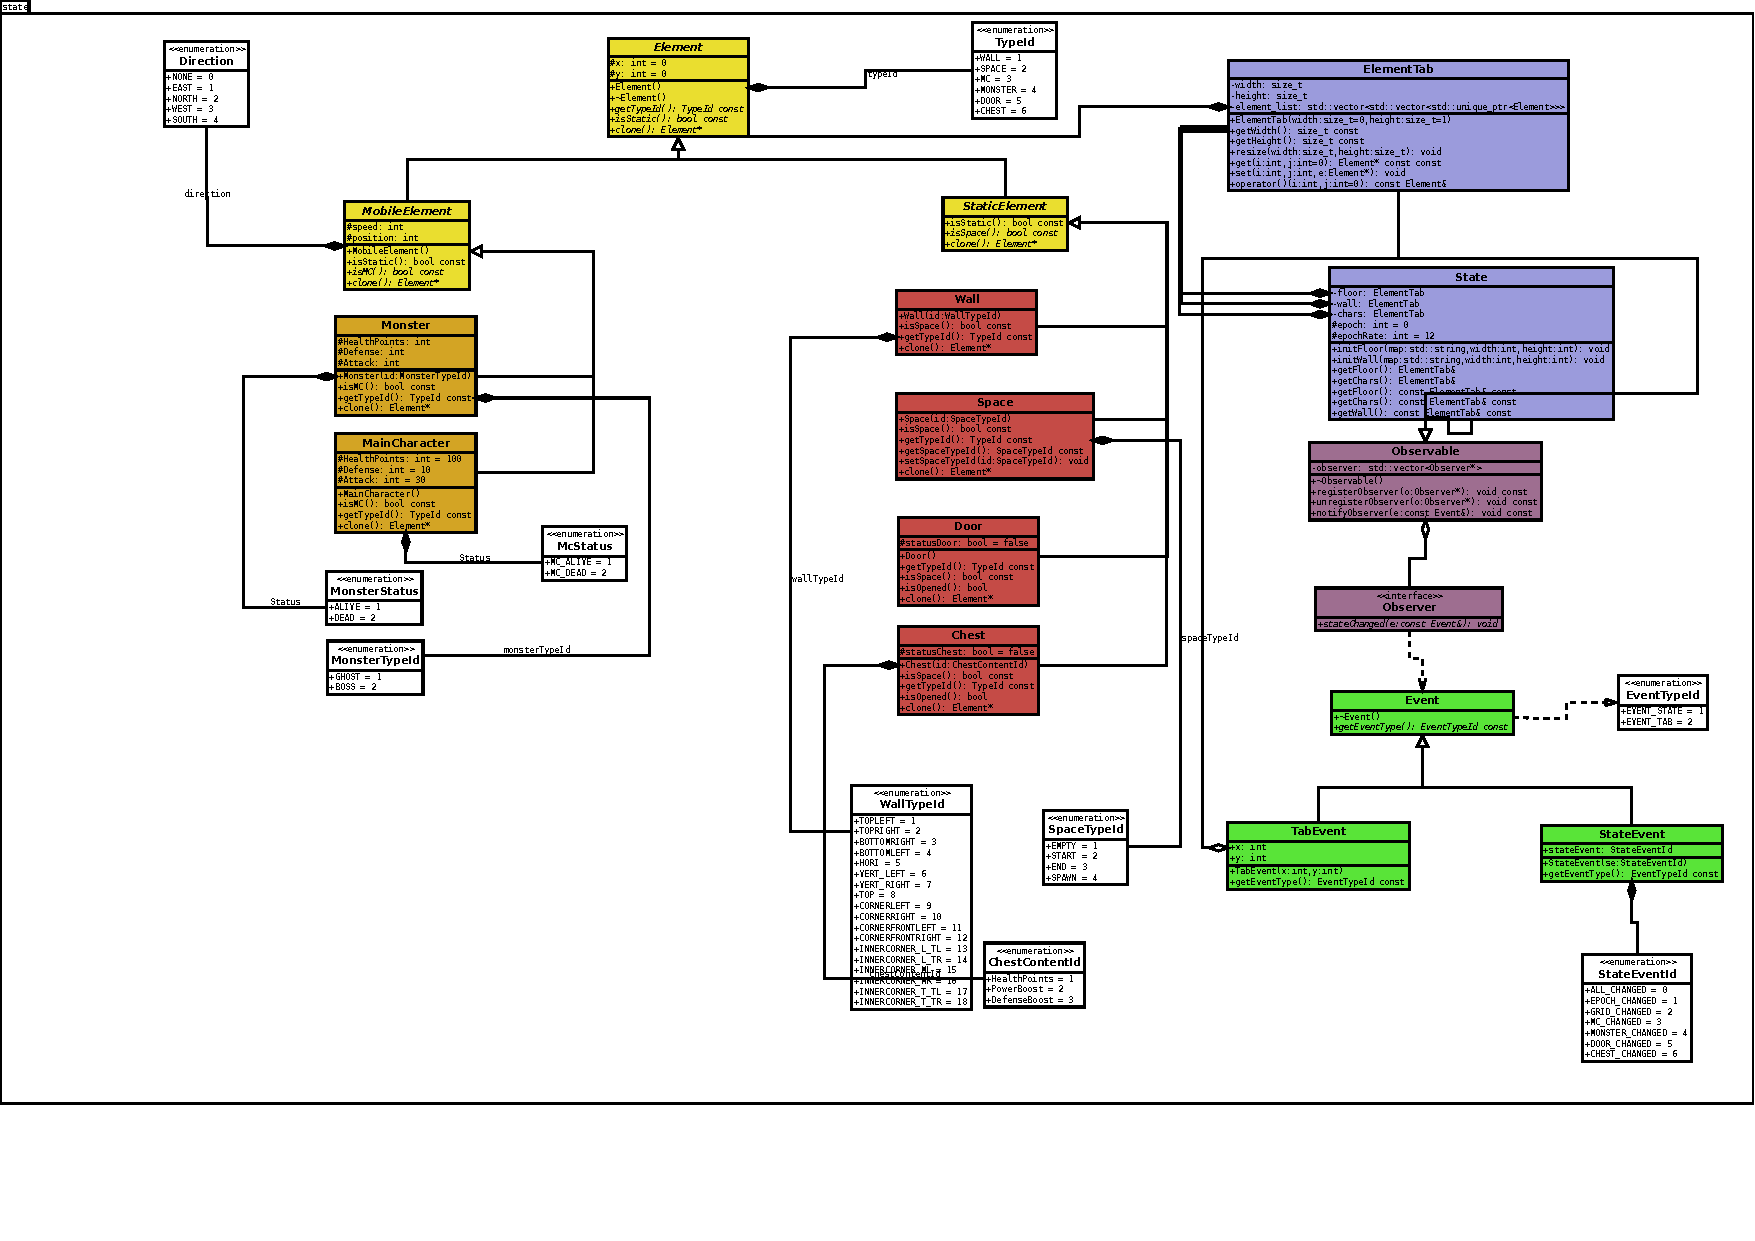
\includegraphics[width=0.9\paperheight]{state.pdf}
%%\caption{\label{uml:state}Diagramme des classes d'état.} 
%%\end{figure}
%%\end{landscape}
%
%\clearpage
%\section{Rendu: Stratégie et Conception}
%
%\subsection{Stratégie de rendu d'un état}
%
%
%\subsection{Conception logiciel}
%
%%\begin{landscape}
%%\begin{figure}[p]
%%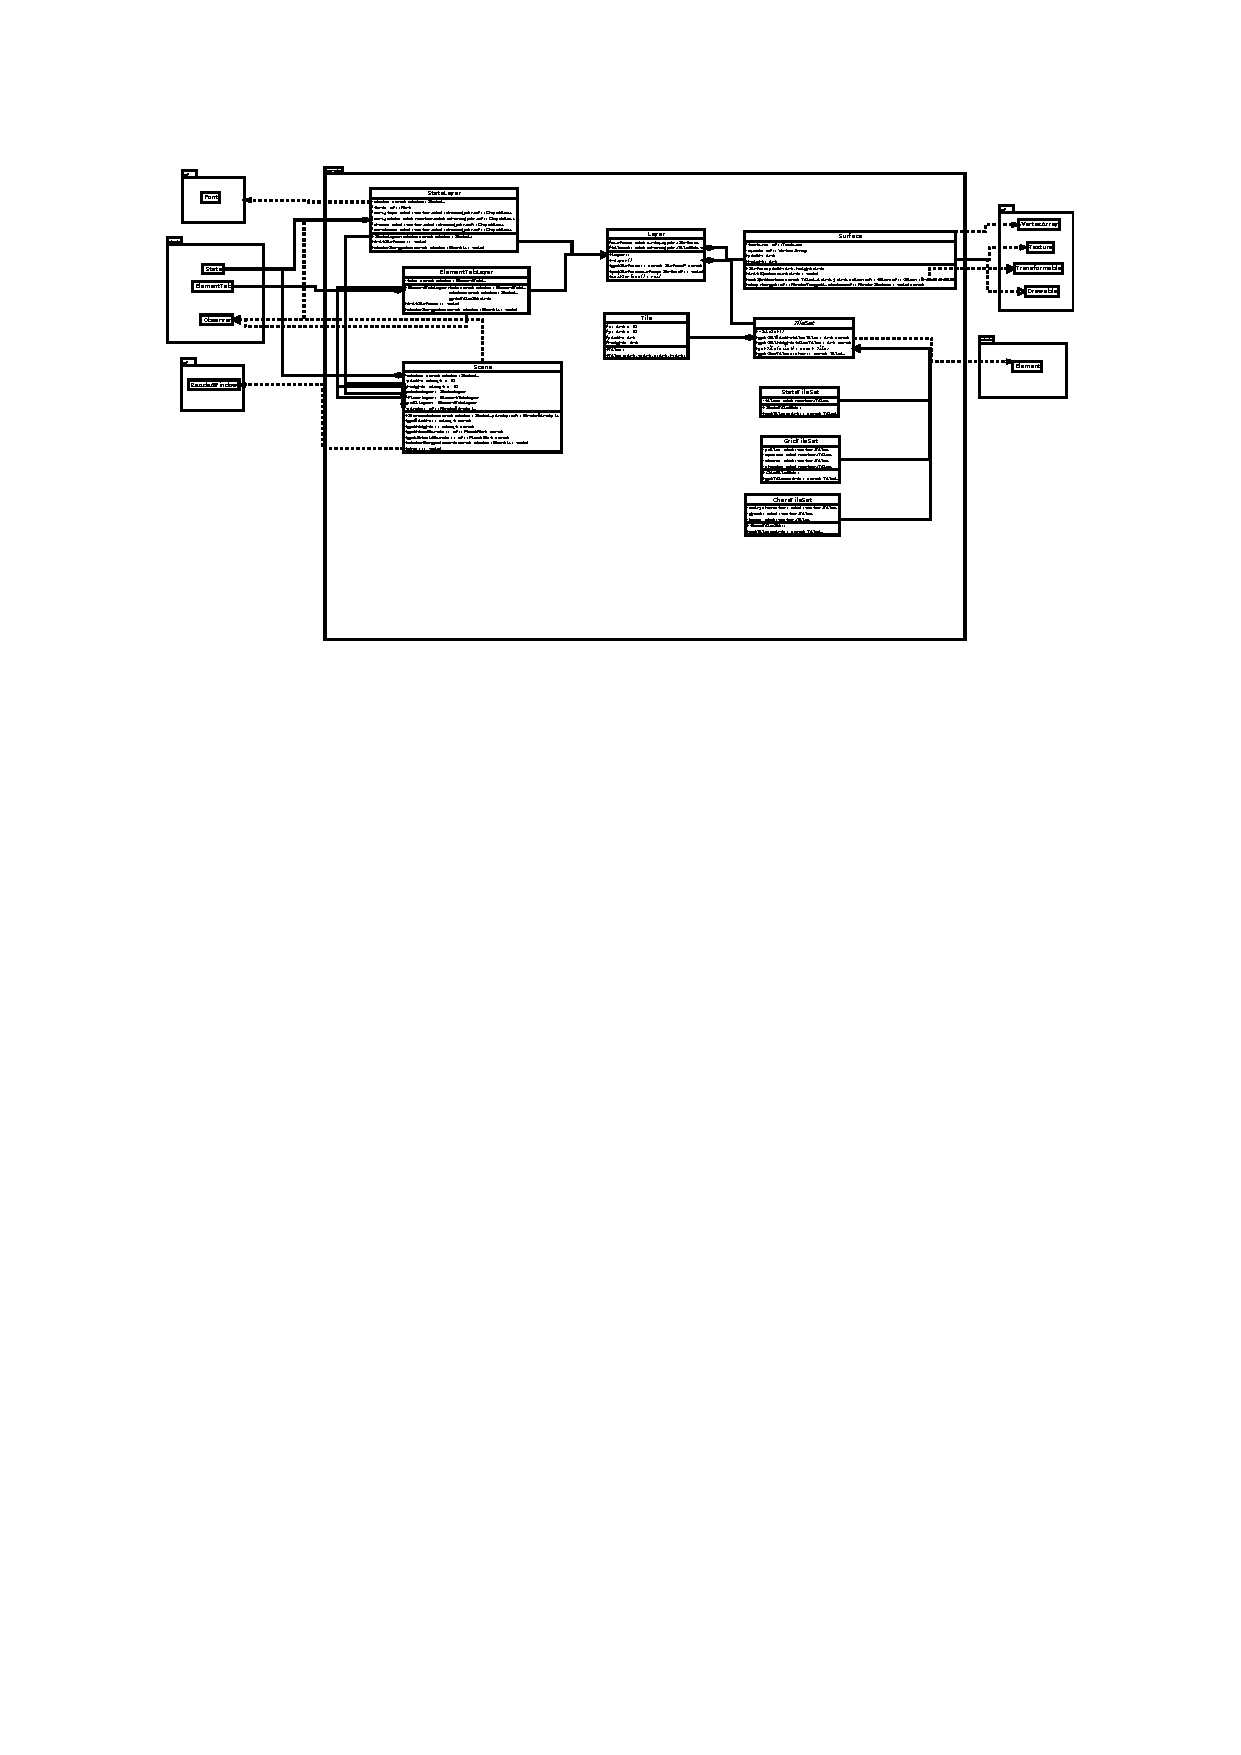
\includegraphics[width=0.9\paperheight]{render.pdf}
%%\caption{\label{uml:render}Diagramme des classes de rendu.} 
%%\end{figure}
%%\end{landscape}
%
%\clearpage
%\section{Règles de changement d'états et moteur de jeu}
%
%\subsection{Règles}
%
%\clearpage
%\subsection{Conception logiciel}
%
%
%%\begin{landscape}
%%\begin{figure}[p]
%%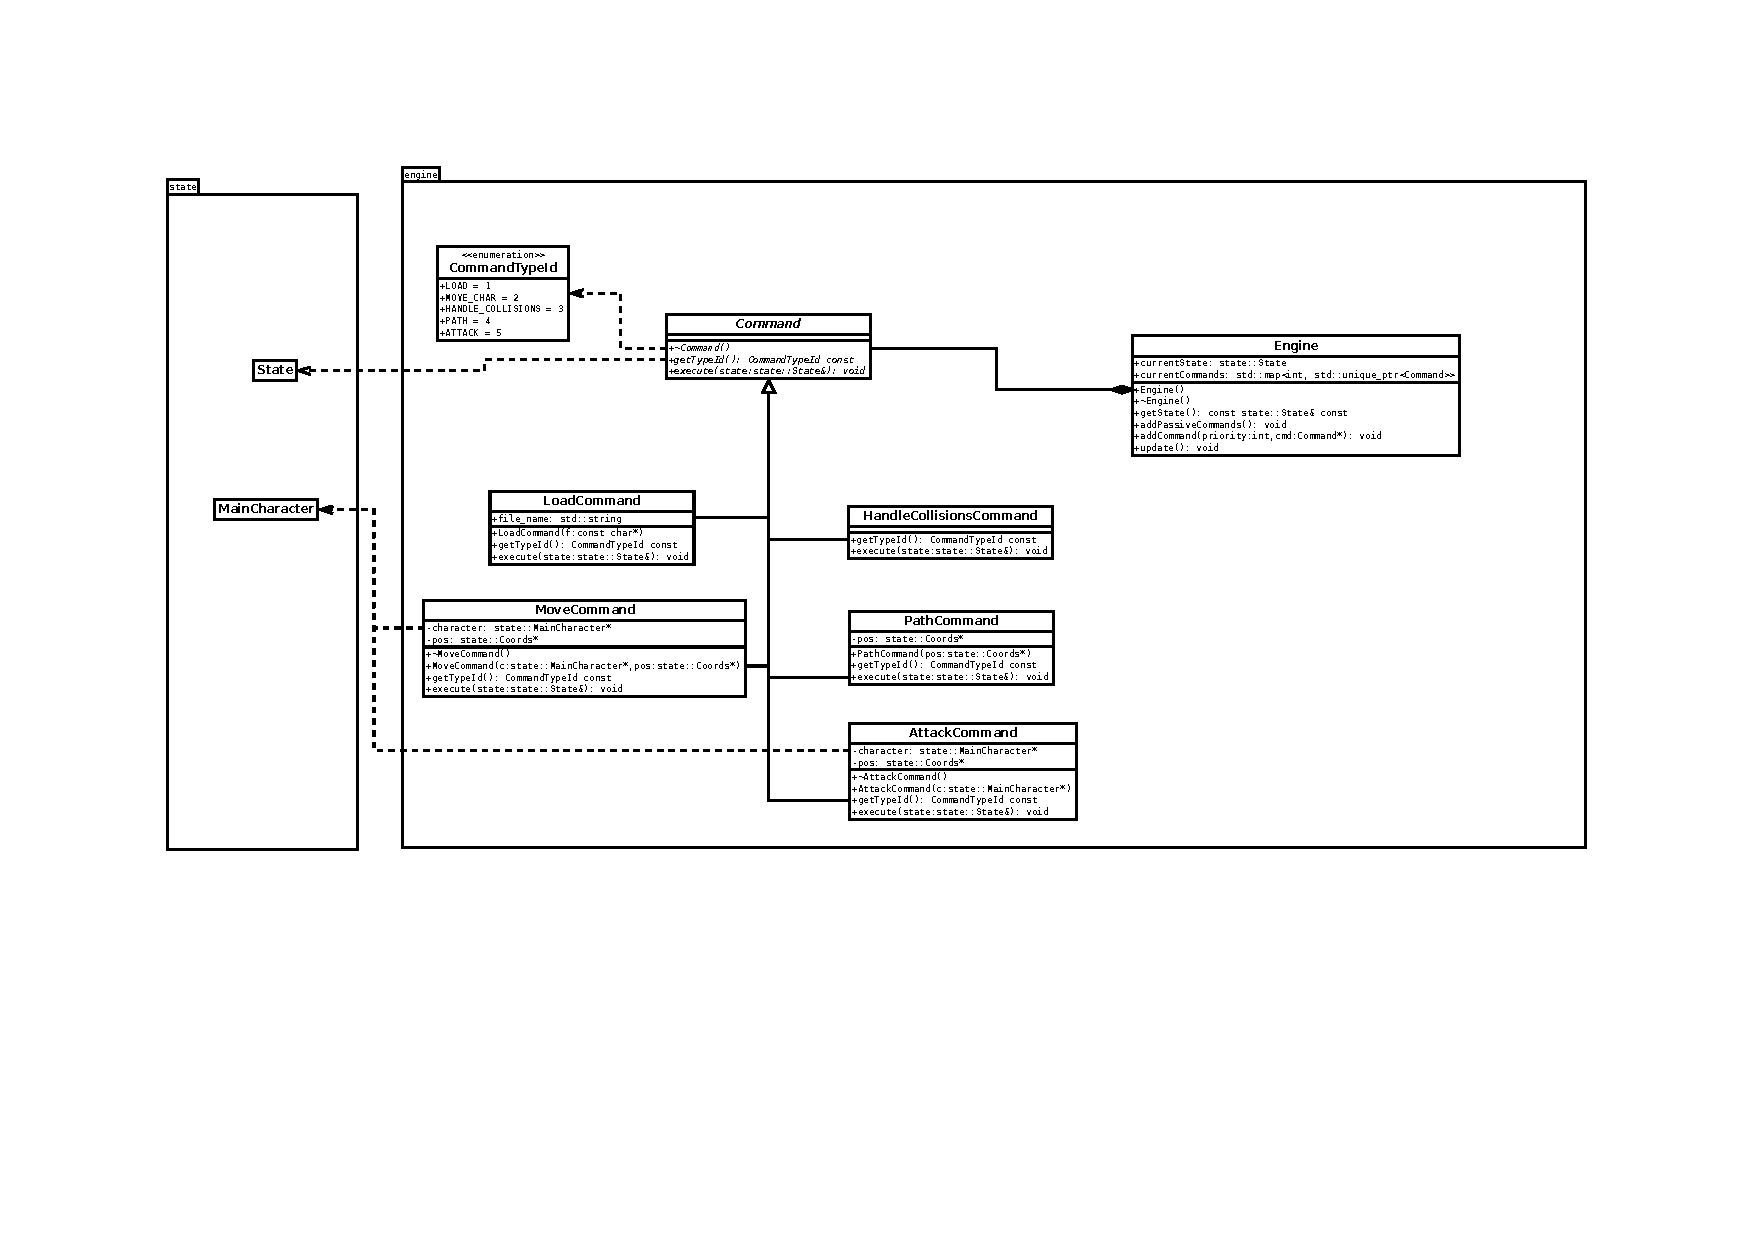
\includegraphics[width=0.9\paperheight]{engine.pdf}
%%\caption{\label{uml:engine}Diagramme des classes de moteur de jeu.} 
%%\end{figure}
%%\end{landscape}
%
%
%\section{Intelligence Artificielle}
%
%\subsection{Stratégies}
%
%\clearpage
%\subsection{Conception logiciel}
%
%
%%\begin{landscape}
%%\begin{figure}[p]
%%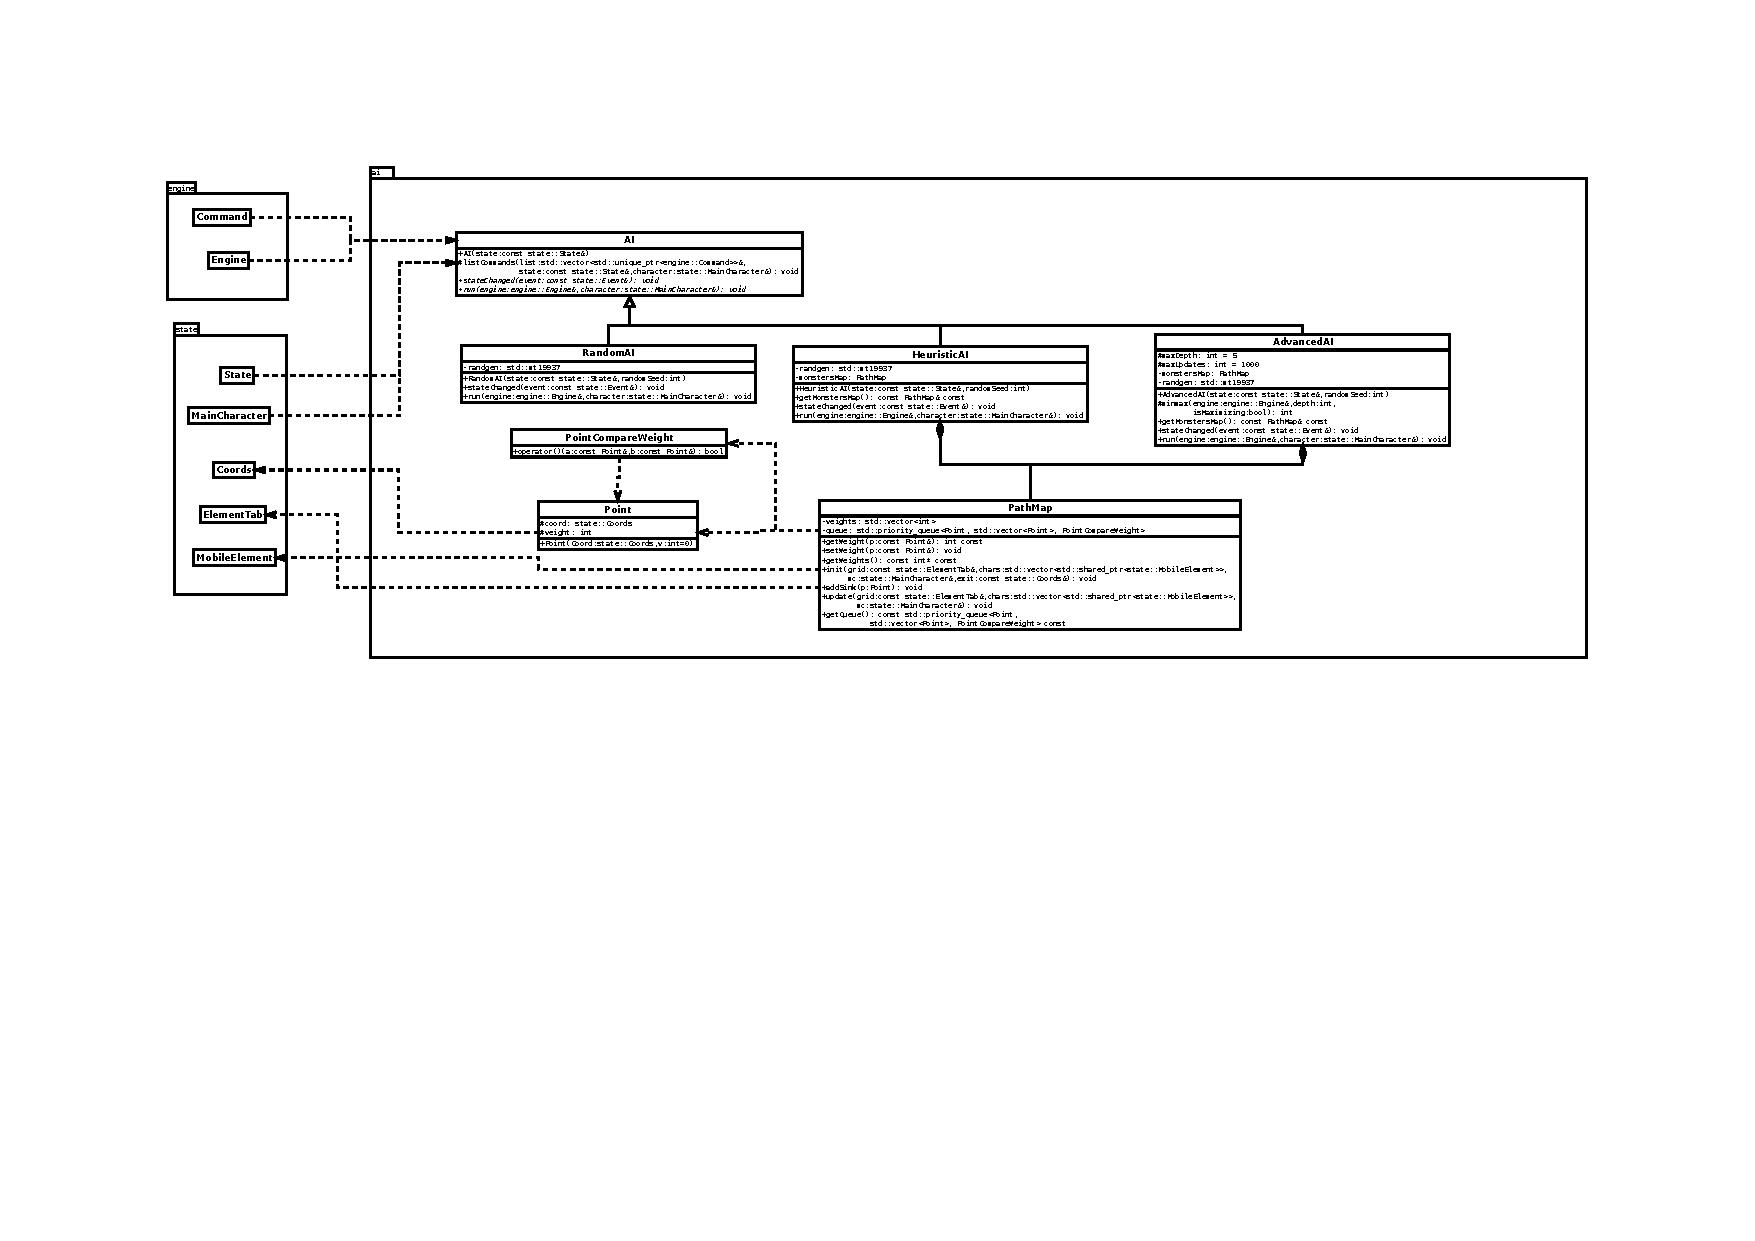
\includegraphics[width=0.9\paperheight]{ai.pdf}
%%\caption{\label{uml:ai}Diagramme des classes d'intelligence artificielle.} 
%%\end{figure}
%%\end{landscape}
%
%
%\section{Modularisation}
%\label{sec:module}
%
%\subsection{Organisation des modules}
%
%\clearpage
%\subsection{Conception logiciel}


%
%\begin{landscape}
%\begin{figure}[p]
%\includegraphics[width=0.9\paperheight]{module.pdf}
%\caption{\label{uml:module}Diagramme des classes pour la modularisation.} 
%\end{figure}
%\end{landscape}
 \addcontentsline{toc}{section}{Sources}
\section*{Sources}

\begin{itemize}
\item[Tiles :] DungeonTiles II \href{https://0x72.itch.io/dungeontileset-ii}{https://0x72.itch.io/dungeontileset-ii} par 0x72
\item[Font :] Pixel Font \href{https://devilsworkshop.itch.io/pixel-font}{https://devilsworkshop.itch.io/pixel-font


} par Ajay Karat | Devil's Work.shop
\end{itemize}

\end{document}
